\definecolor{gt}{RGB}{255 0 255}
\definecolor{cbgl}{RGB}{0 71 145}
\definecolor{err}{RGB}{255 255 0}

% GNUPLOT: LaTeX picture with Postscript
\begingroup
  \makeatletter
  \providecommand\color[2][]{%
    \GenericError{(gnuplot) \space\space\space\@spaces}{%
      Package color not loaded in conjunction with
      terminal option `colourtext'%
    }{See the gnuplot documentation for explanation.%
    }{Either use 'blacktext' in gnuplot or load the package
      color.sty in LaTeX.}%
    \renewcommand\color[2][]{}%
  }%
  \providecommand\includegraphics[2][]{%
    \GenericError{(gnuplot) \space\space\space\@spaces}{%
      Package graphicx or graphics not loaded%
    }{See the gnuplot documentation for explanation.%
    }{The gnuplot epslatex terminal needs graphicx.sty or graphics.sty.}%
    \renewcommand\includegraphics[2][]{}%
  }%
  \providecommand\rotatebox[2]{#2}%
  \@ifundefined{ifGPcolor}{%
    \newif\ifGPcolor
    \GPcolorfalse
  }{}%
  \@ifundefined{ifGPblacktext}{%
    \newif\ifGPblacktext
    \GPblacktexttrue
  }{}%
  % define a \g@addto@macro without @ in the name:
  \let\gplgaddtomacro\g@addto@macro
  % define empty templates for all commands taking text:
  \gdef\gplfronttext{}%
  \gdef\gplfronttext{}%
  \makeatother
  \ifGPblacktext
    % no textcolor at all
    \def\colorrgb#1{}%
    \def\colorgray#1{}%
  \else
    % gray or color?
    \ifGPcolor
      \def\colorrgb#1{\color[rgb]{#1}}%
      \def\colorgray#1{\color[gray]{#1}}%
      \expandafter\def\csname LTw\endcsname{\color{white}}%
      \expandafter\def\csname LTb\endcsname{\color{black}}%
      \expandafter\def\csname LTa\endcsname{\color{black}}%
      \expandafter\def\csname LT0\endcsname{\color[rgb]{1,0,0}}%
      \expandafter\def\csname LT1\endcsname{\color[rgb]{0,1,0}}%
      \expandafter\def\csname LT2\endcsname{\color[rgb]{0,0,1}}%
      \expandafter\def\csname LT3\endcsname{\color[rgb]{1,0,1}}%
      \expandafter\def\csname LT4\endcsname{\color[rgb]{0,1,1}}%
      \expandafter\def\csname LT5\endcsname{\color[rgb]{1,1,0}}%
      \expandafter\def\csname LT6\endcsname{\color[rgb]{0,0,0}}%
      \expandafter\def\csname LT7\endcsname{\color[rgb]{1,0.3,0}}%
      \expandafter\def\csname LT8\endcsname{\color[rgb]{0.5,0.5,0.5}}%
    \else
      % gray
      \def\colorrgb#1{\color{black}}%
      \def\colorgray#1{\color[gray]{#1}}%
      \expandafter\def\csname LTw\endcsname{\color{white}}%
      \expandafter\def\csname LTb\endcsname{\color{black}}%
      \expandafter\def\csname LTa\endcsname{\color{black}}%
      \expandafter\def\csname LT0\endcsname{\color{black}}%
      \expandafter\def\csname LT1\endcsname{\color{black}}%
      \expandafter\def\csname LT2\endcsname{\color{black}}%
      \expandafter\def\csname LT3\endcsname{\color{black}}%
      \expandafter\def\csname LT4\endcsname{\color{black}}%
      \expandafter\def\csname LT5\endcsname{\color{black}}%
      \expandafter\def\csname LT6\endcsname{\color{black}}%
      \expandafter\def\csname LT7\endcsname{\color{black}}%
      \expandafter\def\csname LT8\endcsname{\color{black}}%
    \fi
  \fi
    \setlength{\unitlength}{0.0500bp}%
    \ifx\gptboxheight\undefined%
      \newlength{\gptboxheight}%
      \newlength{\gptboxwidth}%
      \newsavebox{\gptboxtext}%
    \fi%
    \setlength{\fboxrule}{0.5pt}%
    \setlength{\fboxsep}{1pt}%
\begin{picture}(5000.00,2500.00)%
    \gplgaddtomacro\gplfronttext{%
      \put(100,2600){\makebox(0,0){\strut{}{\color{gt}{\rule[0.6mm]{0.5cm}{1.0mm}}} \small Ground truth}}
      \put(2200,2600){\makebox(0,0){\strut{}{\color{cbgl}{\rule[0.6mm]{0.5cm}{1.0mm}}} \small CBGL}}
      \put(4500,2600){\makebox(0,0){\strut{}{\color{err}{\rule[0.6mm]{0.5cm}{1.0mm}}} \small Loc. err. $> 0.5$ m}}

      \colorrgb{0.15,0.15,0.15}%
      %\put(729,440){\makebox(0,0)[r]{\strut{}\small $-2.0$}}%
      \colorrgb{0.15,0.15,0.15}%
      \put(729,796){\makebox(0,0)[r]{\strut{}\small $0.0$}}%
      \colorrgb{0.15,0.15,0.15}%
      %\put(729,953){\makebox(0,0)[r]{\strut{}\small $2.0$}}%
      \colorrgb{0.15,0.15,0.15}%
      \put(729,1309){\makebox(0,0)[r]{\strut{}\small $4.0$}}%
      \colorrgb{0.15,0.15,0.15}%
      %\put(729,1466){\makebox(0,0)[r]{\strut{}\small $6.0$}}%
      \colorrgb{0.15,0.15,0.15}%
      \put(729,1822){\makebox(0,0)[r]{\strut{}\small $8.0$}}%
      \colorrgb{0.15,0.15,0.15}%
      %\put(729,1979){\makebox(0,0)[r]{\strut{}\small $10.0$}}%
      \colorrgb{0.15,0.15,0.15}%
      \put(729,2335){\makebox(0,0)[r]{\strut{}\small $12.0$}}%
      \colorrgb{0.15,0.15,0.15}%
      \put(1310,320){\makebox(0,0){\strut{}\small $5.0$}}%
      \colorrgb{0.15,0.15,0.15}%
      \put(1951,320){\makebox(0,0){\strut{}\small $10.0$}}%
      \colorrgb{0.15,0.15,0.15}%
      \put(2592,320){\makebox(0,0){\strut{}\small $15.0$}}%
      \colorrgb{0.15,0.15,0.15}%
      \put(3233,320){\makebox(0,0){\strut{}\small $20.0$}}%
      \colorrgb{0.15,0.15,0.15}%
      \put(3874,320){\makebox(0,0){\strut{}\small $25.0$}}%
      \put(3876,620){\makebox(0,0){\strut{}\small \scalebox{0.5}{\textit{CSAL} AUTh}}}
    }%
    \gplgaddtomacro\gplfronttext{%
    }%
    \put(0,0){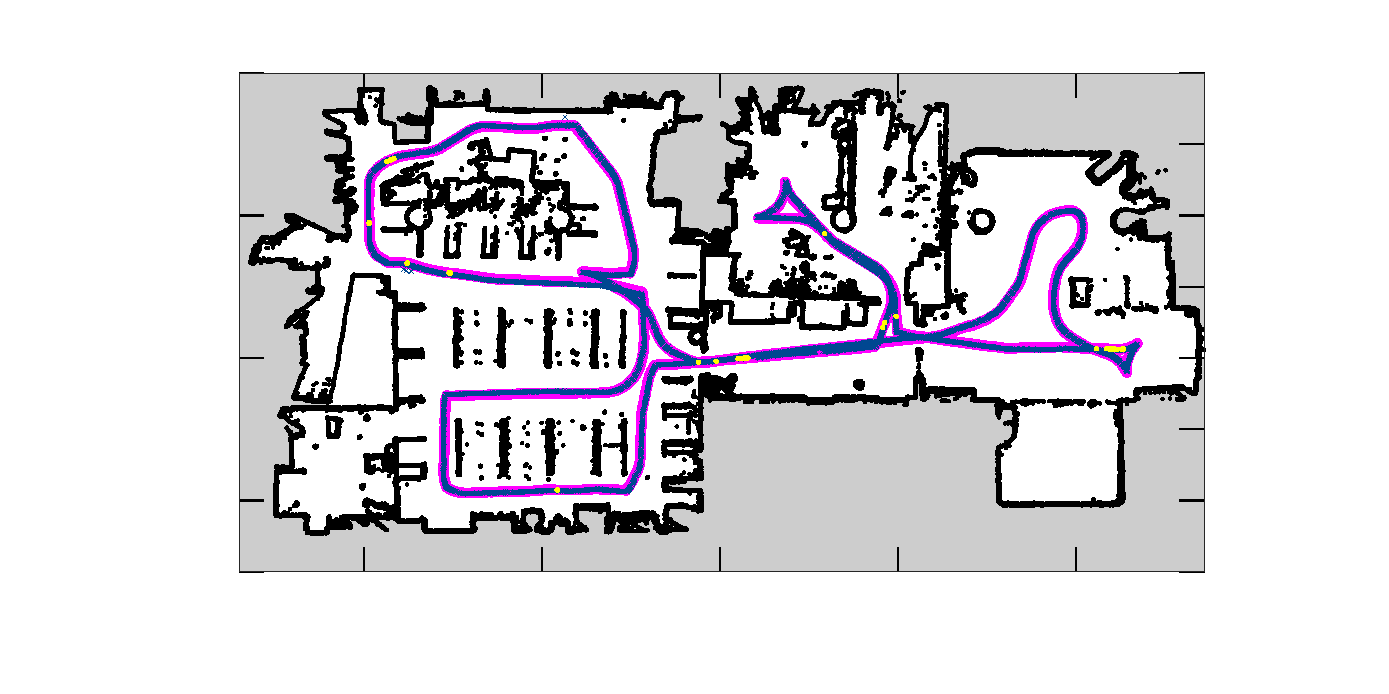
\includegraphics[trim={0 0 0 0.4cm},clip]{./figures/12/trajectory}}%
    \gplfronttext
  \end{picture}%
\endgroup
